\documentclass[a4paper, 12pt]{article}
\usepackage[UTF8]{ctex}
\usepackage{graphicx}
\usepackage{float}
\usepackage[hidelinks]{hyperref}
\begin{document}
\title{Week2 Shell工具和脚本、编辑器(vim)、数据整理}
\author{黄琬晴}
\date{September 2025}
\maketitle
\begin{center}
    本次实验的代码与实验报告上传在github仓库中:\\
    https://github.com/uuukyoo/systools
\end{center}
\pagenumbering{roman}
\tableofcontents
\newpage
\pagenumbering{arabic}


\section{Sell工具和脚本}
\subsection{检查shell是否满足实验要求}
\begin{itemize}
    \item 本课程需要使用类 Unix shell,例如 Bash 或 ZSH。如果您在 Linux 或者 MacOS 上面完成本课程的练习,则不需要做任何特殊的操作。如果您使用的是 Windows,则您不应该使用 cmd 或是 Powershell;您可以使用 Windows Subsystem for Linux 或者是 Linux 虚拟机。使用 echo \$SHELL 命令可以查看您的 shell 是否满足要求。如果打印结果为 /bin/bash 或 /usr/bin/zsh 则是可以的
    
\end{itemize}
echo \$SHELL 命令的结果为/bin/bash,说明我的shell符合本实验的要求
\begin{figure}[H]
    \centering
    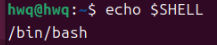
\includegraphics[width=1\linewidth]{shell22.png}
\end{figure}
\subsection{新建文件夹}
\begin{itemize}
    \item 在\verb|/tmp| 下新建一个名为 \verb|missing| 的文件夹

\end{itemize}
\par 使用mkdir命令新建目录,再尝试用cd命令转到\verb|/tmp/missing|文件夹下,尝试成功,说明新建目录成功
\begin{figure}[H]
    \centering
    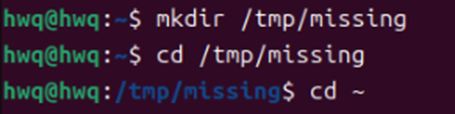
\includegraphics[width=1\linewidth]{shell1.png}
\end{figure}
\subsection{新建文件}
\begin{itemize}
 
    \item \verb|touch| 在 \verb|missing| 文件夹中新建一个叫 \verb|semester| 的文件 
\end{itemize}
在新建文件之前,使用ls命令查看missing文件夹下的文件,此时为空
使用touch 命令在对应目录下新建文件后,再次使用ls查看,此时semester文件出现,说明新建semester文件成功
\begin{figure}[H]
    \centering
    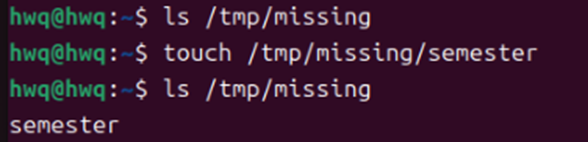
\includegraphics[width=1\linewidth]{shell2.png}
\end{figure}



\subsection{输入输出流重定向到文件}
\begin{itemize}
    \item 将以下内容一行一行地写入 \verb|semester| 文件: 
    \begin{verbatim}
    #!/bin/sh
    curl --head --silent https://missing.csail.mit.edu
    \end{verbatim}
\end{itemize}\par
第一行使用echo和>来将内容覆盖,
第二行使用echo和\verb|>>|来在上一行后追加第二行;并且由于内容中含有有特殊含义的'\#'和'!'字符,所以得使用使用单引号将内容括起来。输入完成后使用cat命令来检查输入的正确性
\begin{figure}[H]
    \centering
    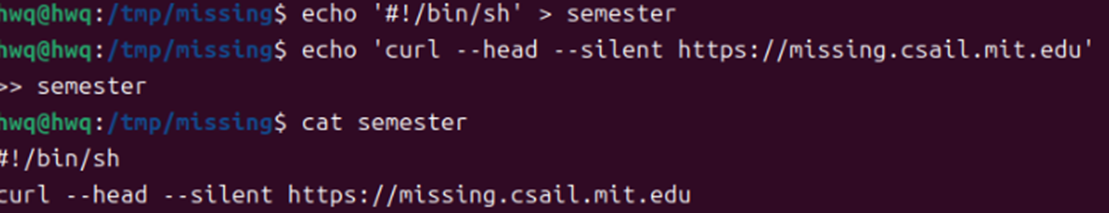
\includegraphics[width=1\linewidth]{shell3.png}
\end{figure}

\subsection{执行文件与权限}
\begin{itemize}
    \item 尝试执行这个文件。例如,将该脚本的路径(\verb|./semester|)输入到您的 shell 中并回车。如果程序无法执行,请使用 \verb|ls| 命令来获取信息并理解其不能执行的原因
\end{itemize}\par
尝试执行
输入./semester尝试执行该文件,发现无法正常执行,显示权限不够
\begin{figure}[H]
    \centering
    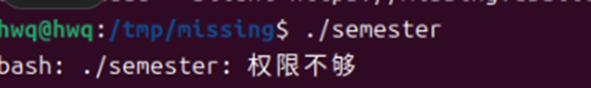
\includegraphics[width=1\linewidth]{shell4.png}
\end{figure}
使用ls -l以长格式查看missing目录下的文件,发现semester 文件没有执行权限,及x权限
\begin{figure}[H]
    \centering
    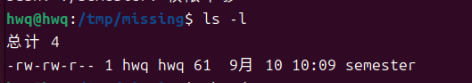
\includegraphics[width=1\linewidth]{shell5.png}
\end{figure}
所以猜想该文件无法正常执行的原因是因为它没有执行权限,用户无法执行没有对该文件的执行权限就无法执行它
\subsection{查看chmod使用手册}
输入man chmod来查看chmod的使用手册
\begin{figure}[H]
    \centering
    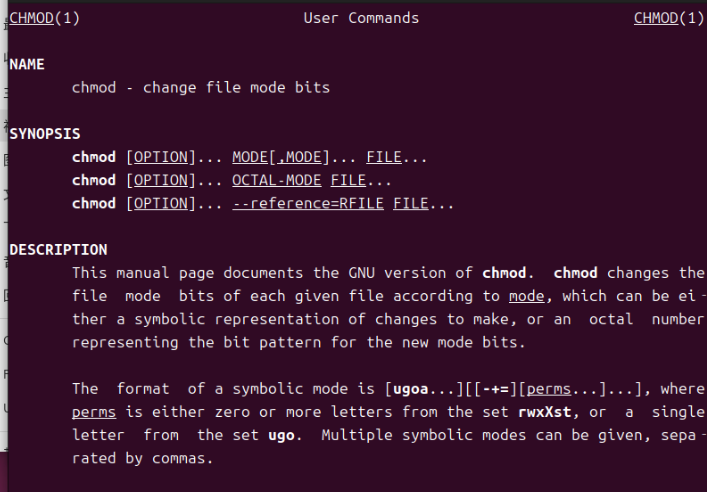
\includegraphics[width=1\linewidth]{shell23.png}
\end{figure}
从使用手册中可以得知,可以使用chmod + x semester命令来为semester文件增加执行权限来解决其无法执行的问题\par
其中的+表示为文件增加权限,与之类似的还有-表示去除权限,=表示将文件对应的用户权限重新设为=后的内容,常见权限有r(read读), w(write写), x(execute执行)等
\subsection{chmod命令与权限}
\begin{itemize}
    \item  使用 \verb|chmod| 命令改变权限,使 \verb|./semester| 能够成功执行,不要使用 \verb|sh semester| 来执行该程序。您的 shell 是如何知晓这个文件需要使用 \verb|sh| 来解析呢? 
\end{itemize}

使用 chmod +x semester,+x表示添加执行权限,semester表示是为semester文件添加执行权限,再次使用ls -l查看,此时就可以发现semester文件已有执行权限
\begin{figure}[H]
    \centering
    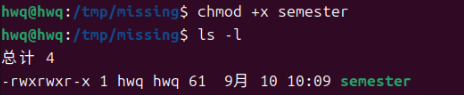
\includegraphics[width=1\linewidth]{shell6.png}
\end{figure}
再次尝试执行,还是无法成功,由显示的curl: not found可知,这此无法成功的原因大概是curl命令未安装
\begin{figure}[H]
    \centering
    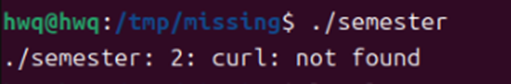
\includegraphics[width=1\linewidth]{shell7.png}
\end{figure}
\subsection{安装未安装的命令}
使用sudo apt install curl命令安装curl命令
\begin{figure}[H]
    \centering
    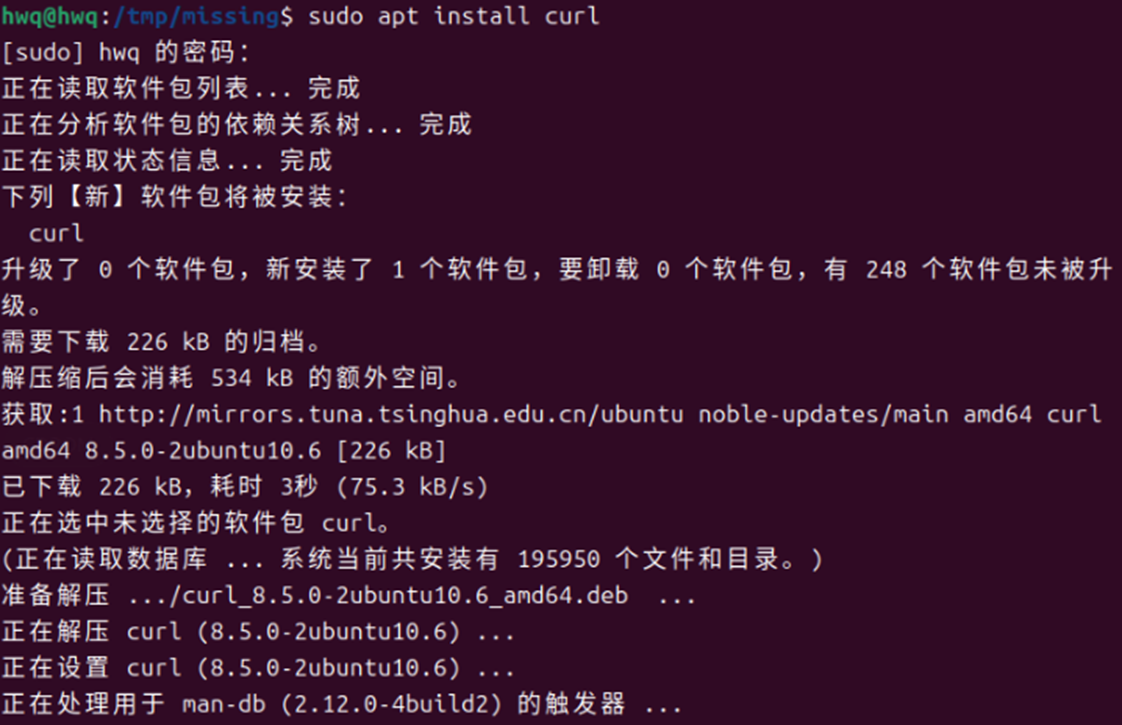
\includegraphics[width=1\linewidth]{shell8.png}
\end{figure}
再次尝试执行,执行成功,现在可以看见执行结果
\begin{figure}[H]
    \centering
    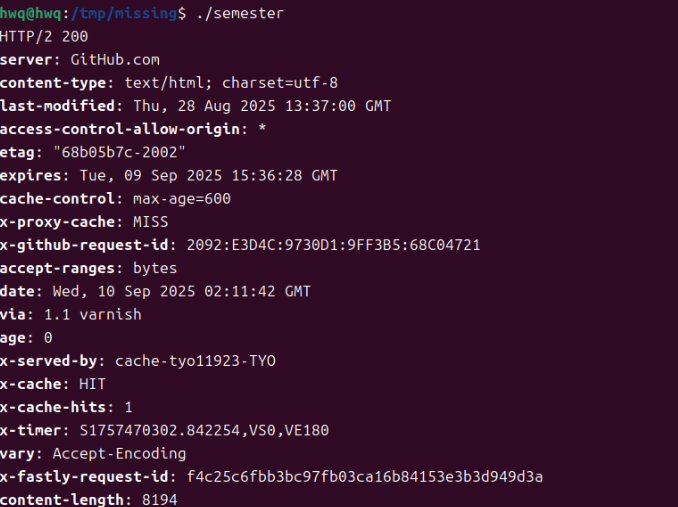
\includegraphics[width=1\linewidth]{shell9.png}
\end{figure}

shell知晓这个文件需要使用 \verb|sh| 来解析,是因为先前我们在编写semester时,将\#!/bin/sh写在了文件的第一行,执行它时,这一行的功能就是告诉操作系统需要用/bin/sh作为解释器,也就是告诉shell这个文件需要使用sh来解析
\subsection{管道}
\begin{itemize}
    \item 使用 \verb||| 和 \verb|>| ,将 \verb|semester| 文件输出的最后更改日期信息,写入主目录下的 \verb|last-modified.txt| 的文件中
\end{itemize}

执行semester文件的结果通过管道传递,由grep过滤出包含last-modified的那一行,将该行内容写入到主目录的last-modified.txt文件中
可以用cat查看文件内容,可以发现与上次执行结果的last-modified相一致
\begin{figure}[H]
     \centering
     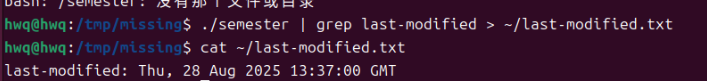
\includegraphics[width=1\linewidth]{shell10.png}
\end{figure}
\subsection{使用ls命令的不同参数来达成不同的目的}
\begin{itemize}
    \item 阅读 man ls ,然后使用 ls 命令进行如下操作:
    \begin{itemize}
        \item 所有文件(包括隐藏文件)
        \item 文件打印以人类可以理解的格式输出 (例如,使用 454M 而不是 454279954)
        \item 文件以最近修改顺序排序
        \item 以彩色文本显示输出结果



 
        
        
        
    \end{itemize}
\end{itemize}\par
使用-a参数可以显示出包括隐藏文件的所有文件,对比ls和ls -a的结果可以看出,显示中多了许多以"."开头的隐藏文件
\begin{figure}[H]
    \centering
    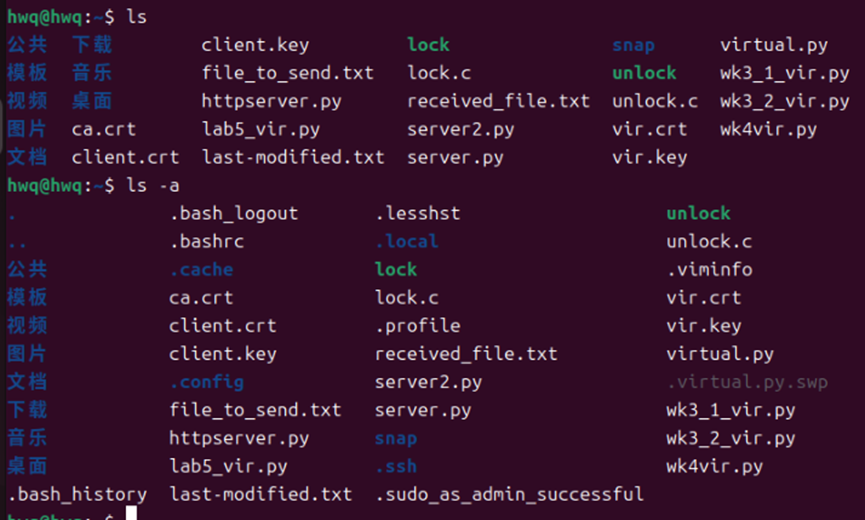
\includegraphics[width=1\linewidth]{shell11.png}
\end{figure}
使用-h参数可以实现文件打印以人类可以理解的格式输出,首先使用-l可以输出文件的详细信息,可以看见此时显示的4096并没有具体的单位
\begin{figure}[H]
    \centering
    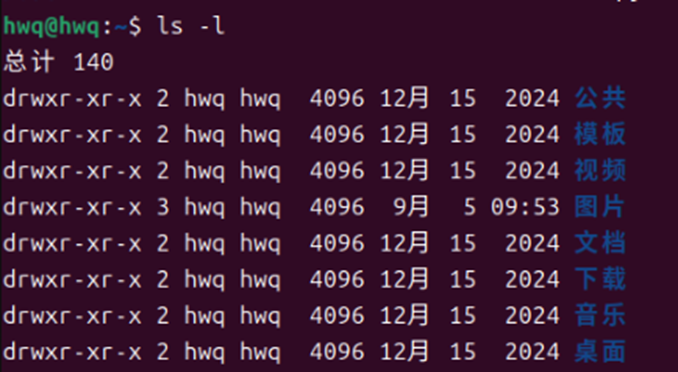
\includegraphics[width=1\linewidth]{shell12.png}
\end{figure}
接着使用了ls -l -h,可以看见4096变成了4.0k,更易于人类理解
\begin{figure}[H]
    \centering
    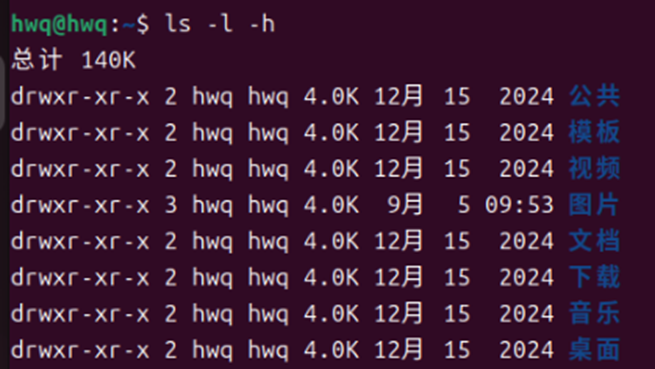
\includegraphics[width=1\linewidth]{shell13.png}
\end{figure}
使用-t可以按修改时间排序
\begin{figure}[H]
    \centering
    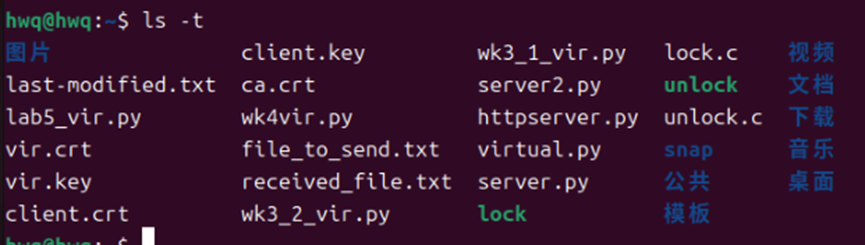
\includegraphics[width=1\linewidth]{shell14.png}
\end{figure}
使用--color=auto参数来以彩色文本输出,但是由于我的shell本来就是以彩色文本输出,所以输出并没有区别
\begin{figure}[H]
    \centering
    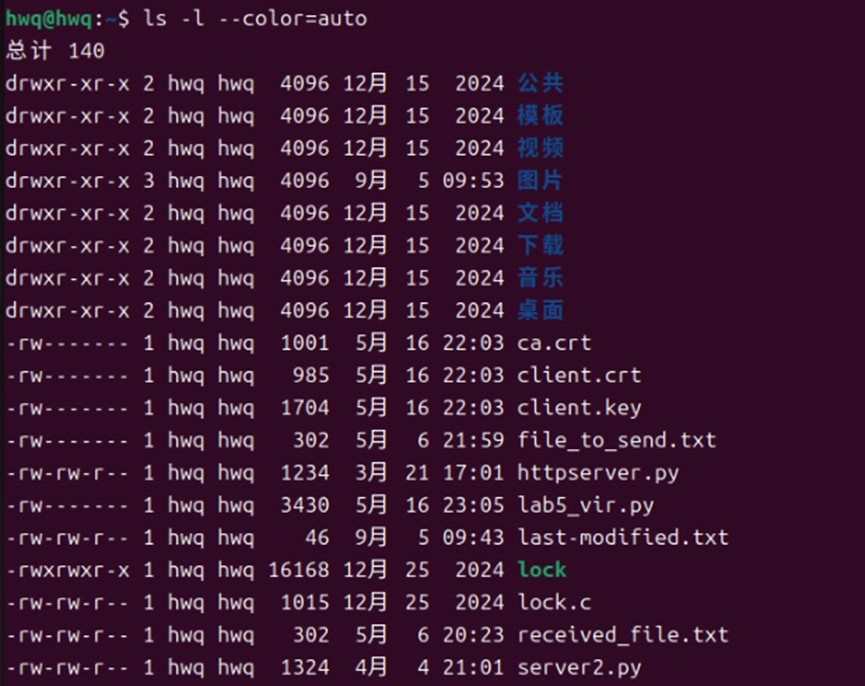
\includegraphics[width=1\linewidth]{shell15.png}
\end{figure}
\subsection{使用bash函数保存工作目录}
\begin{itemize}
    \item 编写两个 bash 函数 marco 和 polo 执行下面的操作。 每当你执行 marco 时,当前的工作目录应当以某种形式保存,当执行 polo 时,无论现在处在什么目录下,都应当 cd 回到当时执行 marco 的目录。 为了方便 debug,你可以把代码写在单独的文件 marco.sh 中,并通过 source marco.sh 命令,(重新)加载函数
\end{itemize}
新建marco.sh文件,内容如下
\begin{figure}[H]
    \centering
    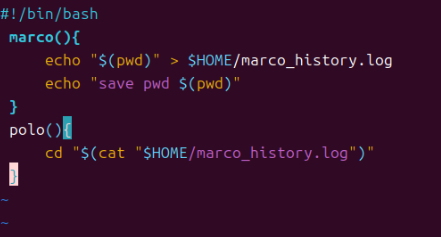
\includegraphics[width=1\linewidth]{shell16.png}
\end{figure}
键入source marco.sh加载函数
\begin{figure}[H]
    \centering
    
\includegraphics[width=1\linewidth]{shell17.png}
\end{figure}
此时输入marco之后,当前工作目录已保存
转到其他目录后输入polo,就转回原来保存的工作目录
\begin{figure}[H]
    \centering
    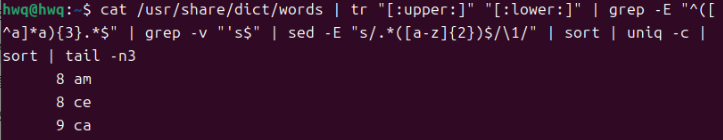
\includegraphics[width=1\linewidth]{image.png}
\end{figure}
\subsection{使用bash函数查找脚本在失败前共运行了多少次}
\begin{itemize}
    \item 假设您有一个命令,它很少出错。因此为了在出错时能够对其进行调试,需要花费大量的时间重现错误并捕获输出。 编写一段 bash 脚本,运行如下的脚本直到它出错,将它的标准输出和标准错误流记录到文件,并在最后输出所有内容。 加分项:报告脚本在失败前共运行了多少次。
    \begin{verbatim}
        #!/usr/bin/env bash

        n=$(( RANDOM % 100 ))

        if [[ n -eq 42 ]]; then
            echo "Something went wrong"
            >&2 echo "The error was using magic numbers"
            exit 1
        fi

        echo "Everything went according to plan"
    \end{verbatim}
\end{itemize}
将题目中给到的脚本保存在buggy.sh中
并将如下内容保存在debug\_for.sh中
\begin{verbatim}
    #!/usr/bin/env bash
    count=0
    echo > out.log

    while true
    do
         ./buggy.sh &>> out.log
        if [[ $? -ne 0 ]]; then
            cat out.log
            echo "failed after $count times"
            break
        fi
        ((count++))

    done
\end{verbatim}
\begin{figure}[H]
    \centering
    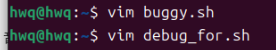
\includegraphics[width=1\linewidth]{shell18.png}
\end{figure}
为它们添加执行权限并执行debug\_for.sh
\begin{figure}[H]
    \centering
    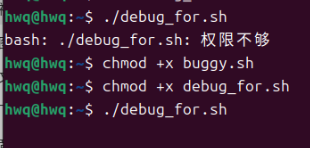
\includegraphics[width=1\linewidth]{shell19.png}
\end{figure}
由运行结果可知在失败之前运行了78次
\begin{figure}[H]
    \centering
    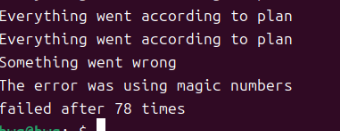
\includegraphics[width=1\linewidth]{shell20.png}
\end{figure}
通过out.log中的记录来验证debug\_for.sh的结果,确实为78次
\begin{figure}[H]
    \centering
    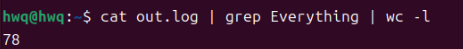
\includegraphics[width=1\linewidth]{shell21.png}
\end{figure}
\section{编辑器vim}
\subsection{完成vimtutor}
\begin{itemize}
    \item 完成 vimtutor。备注:它在一个 80x24(80 列,24 行) 终端窗口看起来效果最好
\end{itemize}
在终端中输入vimturor命令,完成对vim的基本操作的练习
\begin{figure}[H]
    \centering
    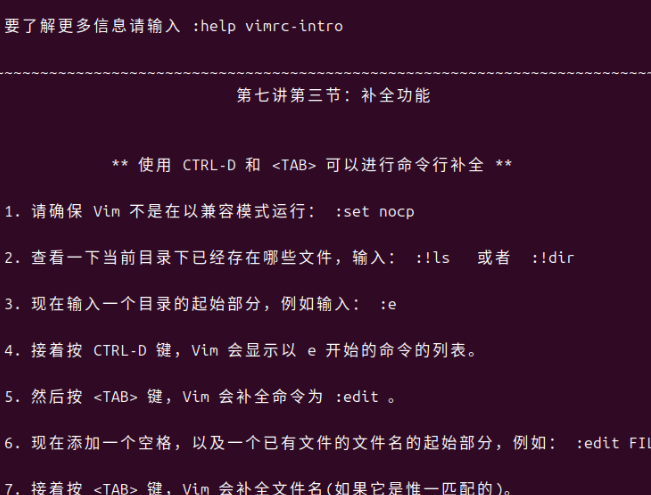
\includegraphics[width=1\linewidth]{vim7.png}
\end{figure}
\subsection{vim意外中断}
若在使用vim编辑文件时意外退出
\begin{figure}[H]
    \centering
    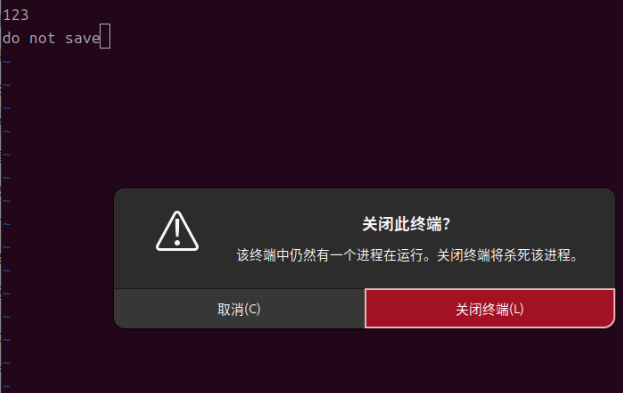
\includegraphics[width=1\linewidth]{vim8.png}
\end{figure}
再次尝试打开文件时就会显示如下
\begin{figure}[H]
    \centering
    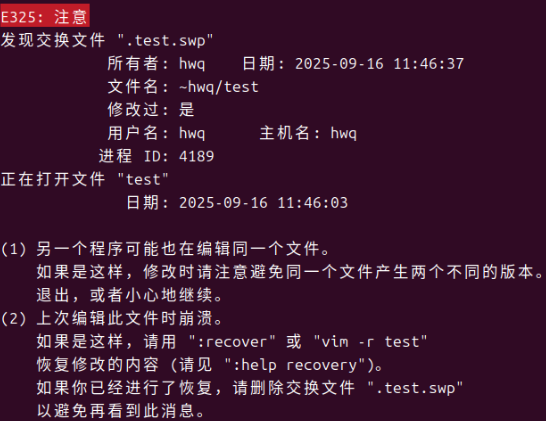
\includegraphics[width=1\linewidth]{vim9.png}
\end{figure}
此时可以输入vim -r test来使用交换文件来恢复原始文件
\begin{figure}[H]
    \centering
    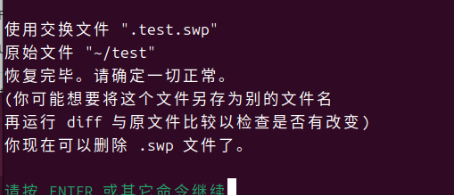
\includegraphics[width=1\linewidth]{vim10.png}
\end{figure}
输入:wq保存即可
\begin{figure}[H]
    \centering
    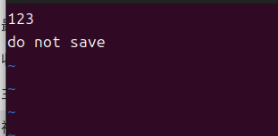
\includegraphics[width=1\linewidth]{vim11.png}
\end{figure}
保存完后即可将交换文件删除
\begin{figure}
    \centering
    
\includegraphics[width=1\linewidth]{vim12.png}
\end{figure}
\subsection{配置\~/.vimrc }
\begin{itemize}
    \item 
下载我们的 \href{https://missing-semester-cn.github.io/2020/files/vimrc}{vimrc},然后把它保存到 \verb|~/.vimrc|。 通读这个注释详细的文件 (用 Vim!), 然后观察 Vim 在这个新的设置下看起来和使用起来有哪些细微的区别。

 
\end{itemize}
将 \verb|~/.vimrc|文件设置为提供的vimrc文件
\begin{figure}[H]
    \centering
    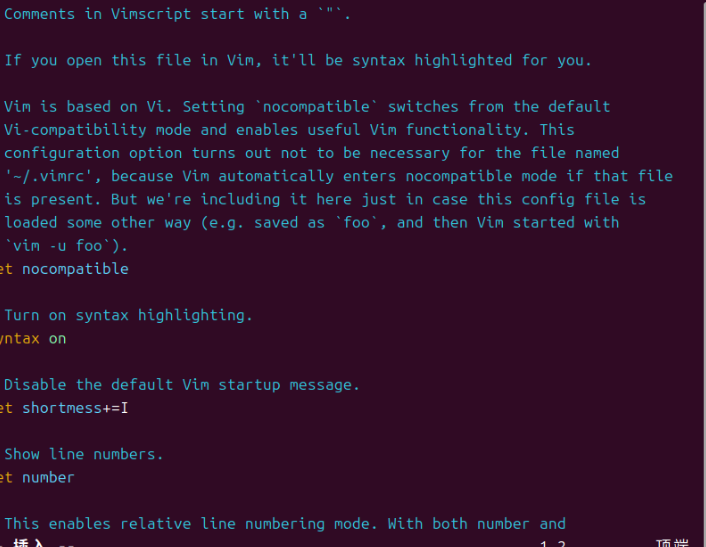
\includegraphics[width=1\linewidth]{vim13.png}
\end{figure}
再次打开vim,比较显著的差别有,方向键被禁用了,鼠标可以定位,下方有如“use J"这样的提示,并且出现了类似行号和状态栏的东西
\begin{figure}[H]
    \centering
    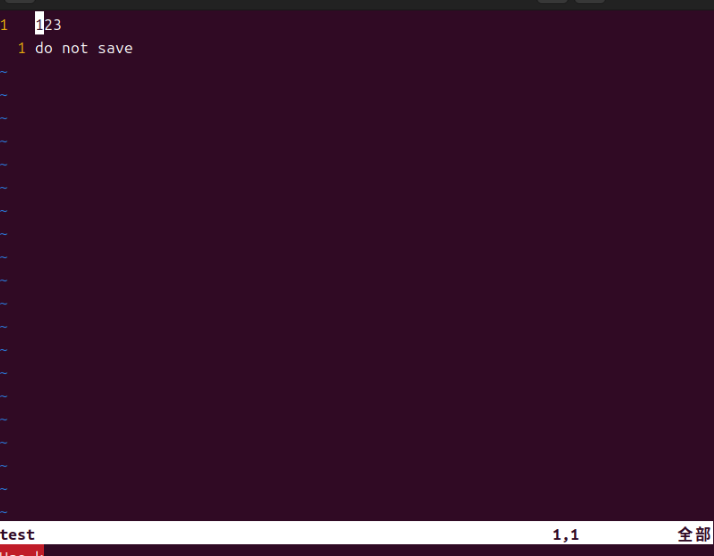
\includegraphics[width=1\linewidth]{vim14.png}

\end{figure}
在看了文件内容后,可以得知它实现的功能:
set nocompatible
关闭 vi 兼容模式,启用 vim 的增强功能

syntax on
打开语法高亮。

set shortmess+=I
禁用 Vim 启动时的欢迎消息。

set number / set relativenumber
打开行号,同时启用相对行号(当前行为实际行号,其余显示相对行号)。

set laststatus=2
始终显示状态栏。

set backspace=indent,eol,start
改善退格键行为,使其能删除缩进、换行符、插入点之前的内容。

set hidden
允许切换到未保存的缓冲区,而不会强制保存。

set ignorecase
搜索默认忽略大小写。

set smartcase
如果搜索词中包含大写字母,则大小写敏感。

set incsearch
输入搜索内容时就实时显示匹配,而不是等回车。

nmap Q <Nop>
禁用 Q 键进入 Ex 模式。

set noerrorbells visualbell t\_vb=
关闭报错提示音和屏幕闪烁。

set mouse+=a
启用鼠标支持

禁止使用方向键(提示使用用 hjkl 来移动)
\subsection{安装和配置一个插件: \href{https://github.com/ctrlpvim/ctrlp.vim}{ctrlp.vim}. }

\begin{enumerate}
    \item 用 \verb|mkdir -p ~/.vim/pack/vendor/start| 创建插件文件夹
    \item 下载这个插件: \verb|cd ~/.vim/pack/vendor/start; git clone https://github.com/ctrlpvim/ctrlp.vim|
    \item 阅读这个插件的 \href{https://github.com/ctrlpvim/ctrlp.vim/blob/master/readme.md}{文档}。 尝试用 CtrlP 来在一个工程文件夹里定位一个文件,打开 Vim, 然后用 Vim 命令控制行开始 \verb|:CtrlP|.
    \item 自定义 CtrlP:添加 \href{https://github.com/ctrlpvim/ctrlp.vim/blob/master/readme.md\#basic-options}{configuration} 到你的 \verb|~/.vimrc| 来用按 Ctrl-P 打开 CtrlP
\end{enumerate}

 创建文件夹,并转到该文件夹下下载该插件
\begin{figure}[H]
    \centering
    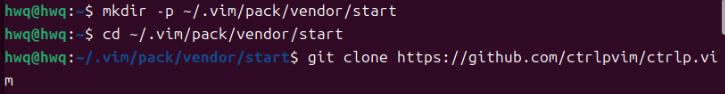
\includegraphics[width=1\linewidth]{vim6.png}
\end{figure}
在\verb|~/.vimrc|中添加如下内容
\begin{figure}[H]
    \centering
    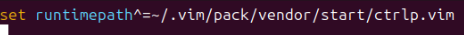
\includegraphics[width=1\linewidth]{vim4.png}
\end{figure}
通过\verb|vim ~/.vim/pack/vendor/start/ctrlp.vim/doc/ctrlp.txt|进入插件的文档目录来阅读该文件的文档
\begin{figure}[H]
    \centering
    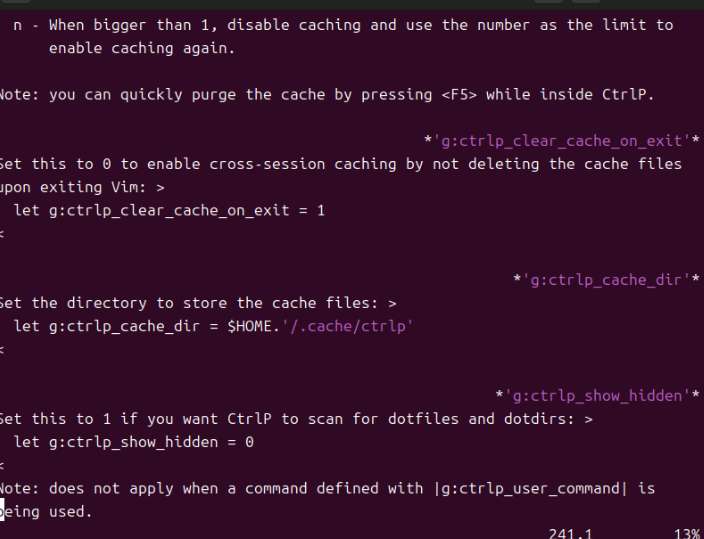
\includegraphics[width=1\linewidth]{vim1.png}
\end{figure}
在vim命令行里输入:CtrlP即可开始使用CtrlP插件的功能
\begin{figure}[H]
    \centering
    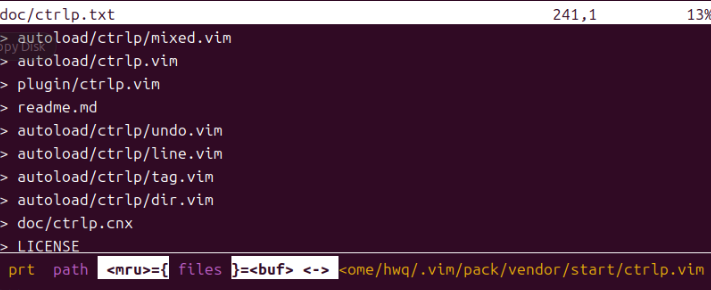
\includegraphics[width=1\linewidth]{vim2.png}
\end{figure}
在\verb|~/.vimrc|中添加如下内容
\begin{figure}[H]
    \centering
    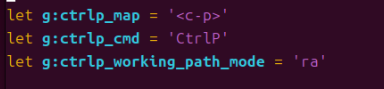
\includegraphics[width=1\linewidth]{vim3.png}
\end{figure}
再次使用vim查看一个文件,此时只需按下Ctrl+P即可打开文件查找
\begin{figure}[H]
    \centering
    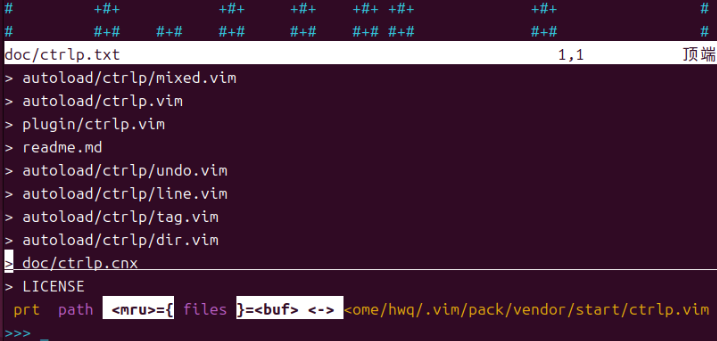
\includegraphics[width=1\linewidth]{vim5.png}
\end{figure}:
\section{数据整理}
\subsection{sed能否原地替换}
\begin{itemize}
    \item 进行原地替换听上去很有诱惑力,例如:
sed s/REGEX/SUBSTITUTION/ input.txt > input.txt。
但是这并不是一个明智的做法,为什么呢?还是说只有 \verb|sed| 是这样的?
查看 \verb|man sed| 来完成这个问题 

\end{itemize}
因为在运行sed s/REGEX/SUBSTITUTION/ input.txt > input.txt时,>input.txt会在sed启动前就执行,所以在sed启动前input.txt就已清空,当sed再尝试读取时,input.txt就已是空文件,所以结果只能为空而无法得到正确的结果,并且还会丢失原来的input.txt文件的内容\par
并且不只是sed有这个问题,输出重定向会先将目标文件清空,所以任何的类似的原地替换的命令都会导致文件清空无法得到正确结果,如
\begin{verbatim}
    grep foo file.txt > file.txt  
    awk '{print $1}' file.txt > file.txt

\end{verbatim}
等指令都是如此
\subsection{开机时间统计}
\begin{itemize}
    \item 找出您最近十次开机的开机时间平均数、中位数和最长时间。
\end{itemize}
编写脚本getlog.sh如下,来获取最近十次的开机时间
\begin{figure}[H]
    \centering
    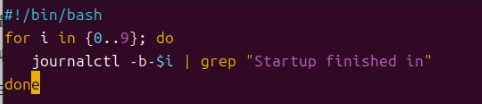
\includegraphics[width=1\linewidth]{data1.png}
\end{figure}
将执行结果存入到starttime.txt中
\begin{figure}[H]
    \centering
    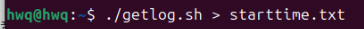
\includegraphics[width=1\linewidth]{data2.png}
\end{figure}
查找出最长时间,最短时间,平均数中位数分别为:27.067s, 25.056s, 25.8622s, 26.051s
\begin{figure}[H]
    \centering
    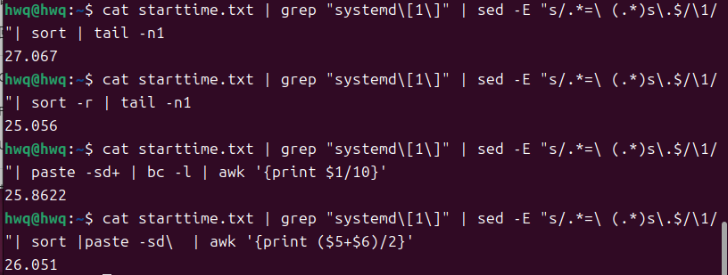
\includegraphics[width=1\linewidth]{data3.png}
\end{figure}
\subsection{统计近三次开机的不同}
\begin{itemize}
    \item 查看之前三次重启启动信息中不同的部分
\end{itemize}
将上一题的getlog.sh改为获得近三次启动信息
\begin{figure}[H]
    \centering
    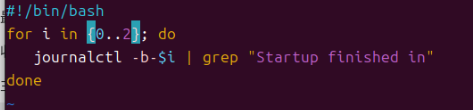
\includegraphics[width=1\linewidth]{data4.png}
\end{figure}
将近三次启动信息存储到文件last3.txt中,查找除时间戳之外的不同
\begin{figure}[H]
    \centering
    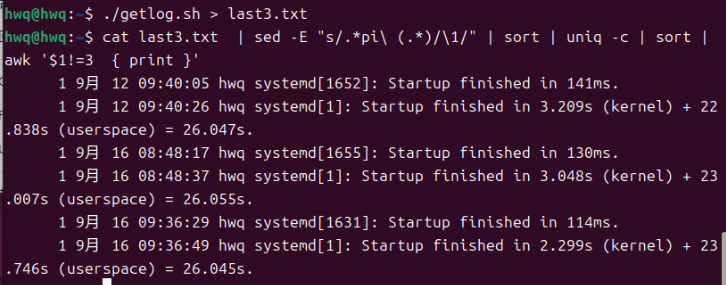
\includegraphics[width=1\linewidth]{data5.png}
\end{figure}
\subsection{统计words文件}
\begin{itemize}
    \item 统计 words 文件 (/usr/share/dict/words) 中包含至少三个 a 且不以 's 结尾的单词个数。这些单词中,出现频率前三的末尾两个字母是什么? sed 的 y 命令,或者 tr 程序也许可以帮你解决大小写的问题。共存在多少种词尾两字母组合?

\end{itemize}
查找包含至少三个a且不是以's结尾的单词个数,为854个
\begin{figure}[H]
    \centering
    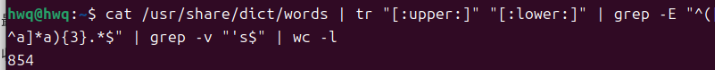
\includegraphics[width=1\linewidth]{data7.png}
\end{figure}
频率前三的末尾两个字母分别是am, ce, ca
\begin{figure}[H]
    \centering
    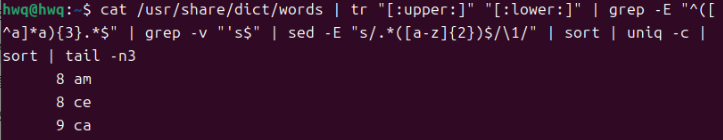
\includegraphics[width=1\linewidth]{data8.png}
\end{figure}
共存在112种词尾两字母组合
\begin{figure}[H]
    \centering
    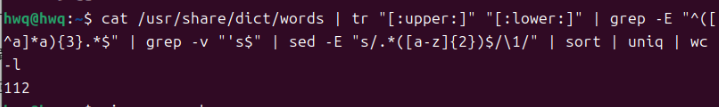
\includegraphics[width=1\linewidth]{data9.png}
\end{figure}
\section{实验心得}
通过本次实验我学习了shell的使用方法,如何自定义vim编辑器的功能、插件等,还学习了基本的数据整理方法\par
之前我对它们的了解仅仅在大概会用但是不是很了解的程度上,每次如果遇到了什么记不住的指令或者不知道如何解决的问题都是现用现搜,通过本次学习,本来只在我大脑里有模糊概念的知识变得轮廓清晰了起来
\end{document}
